% This must be in the first 5 lines to tell arXiv to use pdfLaTeX, which is strongly recommended.
\pdfoutput=1
% In particular, the hyperref package requires pdfLaTeX in order to break URLs across lines.

\documentclass[11pt]{article}

% Remove the "review" option to generate the final version.
\usepackage[review]{EMNLP2023}

% Standard package includes
\usepackage{times}
\usepackage{latexsym}

% For proper rendering and hyphenation of words containing Latin characters (including in bib files)
\usepackage[T1]{fontenc}
% For Vietnamese characters
% \usepackage[T5]{fontenc}
% See https://www.latex-project.org/help/documentation/encguide.pdf for other character sets

% This assumes your files are encoded as UTF8
\usepackage[utf8]{inputenc}

% This is not strictly necessary, and may be commented out.
% However, it will improve the layout of the manuscript,
% and will typically save some space.
\usepackage{microtype}

% This is also not strictly necessary, and may be commented out.
% However, it will improve the aesthetics of text in
% the typewriter font.
\usepackage{inconsolata}


% If the title and author information does not fit in the area allocated, uncomment the following
%
%\setlength\titlebox{<dim>}
%
% and set <dim> to something 5cm or larger.

\title{Instructions for EMNLP 2023 Proceedings}

% Author information can be set in various styles:
% For several authors from the same institution:
% \author{Author 1 \and ... \and Author n \\
%         Address line \\ ... \\ Address line}
% if the names do not fit well on one line use
%         Author 1 \\ {\bf Author 2} \\ ... \\ {\bf Author n} \\
% For authors from different institutions:
% \author{Author 1 \\ Address line \\  ... \\ Address line
%         \And  ... \And
%         Author n \\ Address line \\ ... \\ Address line}
% To start a seperate ``row'' of authors use \AND, as in
% \author{Author 1 \\ Address line \\  ... \\ Address line
%         \AND
%         Author 2 \\ Address line \\ ... \\ Address line \And
%         Author 3 \\ Address line \\ ... \\ Address line}

\author{First Author \\
  Affiliation / Address line 1 \\
  Affiliation / Address line 2 \\
  Affiliation / Address line 3 \\
  \texttt{email@domain} \\\And
  Second Author \\
  Affiliation / Address line 1 \\
  Affiliation / Address line 2 \\
  Affiliation / Address line 3 \\
  \texttt{email@domain} \\}

\begin{document}
\maketitle
\begin{abstract}
Natural language processing (NLP) techniques have increased substantially in performance and can potentially automate some areas of legal reasoning and writing. However, increased performance has come at the cost of increased opacity of the models. XAI has been developed to combat this opacity. Nevertheless, it is unclear how such explanations should be evaluated and whether these explanations are effective because effectiveness depends on the varying purposes and end-users of the explanations. Separately, the stakeholders of data privacy regulation (i.e. organisations, data privacy regulatory authorities, and consumers of data services) can benefit particularly from the use of XAI. Hence, this capstone fills a gap in research by evaluating the effectiveness of XAI within the context of data privacy.

This capstone trains and reports the performance of machine learning classifiers that detect data practices in PlayStore apps' data privacy policies. Then, an XAI technique, LIME, is applied on these models to produce explanations of classifications of selected data practices. Finally, the explanations are evaluated by human evaluation using a survey which uniquely utilises varied types of questions to measure different values linked to explanability (effectiveness, risk, fairness and trust) from the perspective of different stakeholders of data privacy. In terms of model performance, I achieve a 5-class weighted average F1 score of 66\% using SVC with Tf-IDF. In terms of human evaluation, after viewing the explanations, respondents reported a statistically significant decrease in overall trust and understandability of the models, amongst other more specific findings.
\end{abstract}

\section{Motivation and significance}
A question was posed in 2017: "Will there be a software service for the generation of explanations and arguments in law that will assist in structuring explanations of answers and supportive legal arguments?" \cite{ashley_2017}. This question seems close to getting an answer in 2023 with the release of ChatGPT \cite{openai} to the general public. Consider the following response from ChatGPT:  

% \begin{figure}[!ht]
% 	\centering
% 	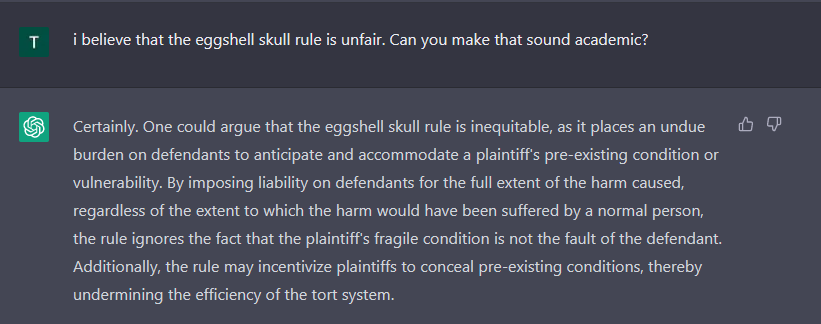
\includegraphics[width=1\linewidth]{figures/chatgpt3.png}
% 	\caption{Conversation with ChatGPT about the egg-shell skull rule.}   
%   \label{fig:chatgpt}
% \end{figure}

Indeed, GPT-4, successor of ChatGPT and released a mere 4 months after ChatGPT, scored on the 90th percentile on the Uniform Bar Exam which is significantly in excess of the passing mark to practice law in the US \cite{katz2023gpt}.

ChatGPT and GPT-4 are the most recent AI models that uses advanced natural language processing (NLP). NLP is a branch of AI that gives computers the ability to understand text and spoken words as how human beings would understand \cite{ibm_nlp}. While NLP techniques have substantially increased in performance in recent years, it has come at the cost of the explainability of their predictions because of models that are architecturally more complex and opaque \cite{zini2022}. This issue of explainability is exemplified by the last question I posed to ChatGPT about its view on the egg-shell skull rule:

% \begin{figure}[!ht]
% 	\centering
% 	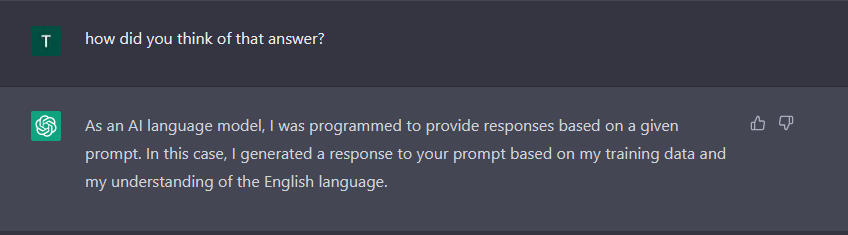
\includegraphics[width=1\linewidth]{figures/chatgpt2.png}
% 	\caption{Conversation with ChatGPT about the egg-shell skull rule.}   
%   \label{fig:chatgpt2}
% \end{figure}

ChatGPT does not seem to be able to explain its views like how a typical human would. Further prompting led ChatGPT to provide a list of academic papers that support its view. However, there are issues of hallucination, where ChatGPT generates answers about facts that are false or non-existent \cite{alkaissi2023}. This lack of explainability (and potential inaccuracies of the explanations) could significantly hinder NLP's greater adoption within the legal industry because the lawyer that uses these models ultimately bear the legal responsibility of ensuring that the analysis is legally sound. In Singapore, a legal practitioner must act with reasonable diligence and competence in the provision of services to the client\footnote{According to r5(2)(c) of the Legal Profession (Professional Conduct) Rules 2015.}. A lawyer that relies on the analysis of legal tech tools but does not understand how the analysis was produced could be considered lacking in diligence and competence.

Nevertheless, the intersection in skillset between data science and legal analysis is still nascent and it is unrealistic to expect all legally trained personnel to be proficient in data science to the extent required to understand the logic of machine learning models without aid. Thus, eXplainable AI (XAI) techniques and research have been rising in popularity and has most recently found its way into the the EU's proposed AI Act that places explainability requirements on AI providers \cite{gyevnar2023}. XAI refers to methods that attempt to help the end user of a model understand how it arrives at its result \cite{danilevsky2020}, which reduces the model's opacity. XAI can therefore bridge the gap between the lawyer and the data scientist by using XAI techniques to explain the predictions of AI models used in legal decision making. 

However, there is not much consensus about what "explainable" means. While the general agreed upon goal of XAI is to "completely, accurately and clearly quantify the [model's] logic", there is no consistent use of the terms "explainability", "interpretability" and "transparency" \cite{danilevsky2020}. Interpretability is sometimes used to describe the model's internal logic and explainability as the ability of the user to understand that logic. However, explainability is also described as techniques to explain the model's logic post-hoc without necessarily being representative of the model's true decision \cite{rosenfeld2021}. Though the AI Act frequently refers to different levels of transparency, there is no explicit definition of transparency. Transparency could involve mandatory disclosure of an AI system used in decision-making which is a much broader concept than transparency used in current XAI literature that covers only the algorithmic process \cite{gyevnar2023}. In this capstone, I use explainability, interpretability, understandability and transparency interchangeably to refer to the overall goal of XAI as stated above.

Another area of XAI is differentiating what explainability means to different users of the model who have different purposes for the explanations. For example, what could be explainable to data scientists may not be explainable to laypersons. While data scientists may find that more technical details about the model would make the model more understandable, laypersons might be more confused if too many details are provided \cite{rosenfeld2021}. Therefore, assessing the effectiveness of XAI is highly dependent on the specific context and needs of the users. 

In this capstone, XAI is assessed within the context of data privacy. The widespread collection and use of data by organisations in recent years has led to an increase of regulations governing data privacy, with 145 countries having enacted data protection legislation in 2021 \cite{gstrein2022}. With more sophisticated regulation comes increased difficulties for organisations to ensure that they are complying with these regulations, and for governments to enforce them. Given that explainability is context and user dependent, the following explains why XAI is important to the three different stakeholders in data privacy: the consumer, organisation and state.

For the consumer, it is uncontroversial that data privacy policies on websites and software are rarely read, and even if they are read, consumers are unlikely to fully understand them because of the use of extensive legalese. The ease of reading data privacy policies was measured to be roughly the same as compared to academic articles such as the Harvard Law Review. The average policy takes 17 minutes to read, and the annual reading time per consumer is more than 400 hours which is more than an hour per day\footnote{Assuming that a consumer visits 1462 unique websites each year.} \cite{wagner2022privacy}. This increasing unreadability of data privacy policies poses a significant challenge to the effectiveness of data privacy regulation given that the current model of regulation depends on the consumer giving consent that is informed and freely given \cite{mantelero_2014}. Combined with the increasing collection and use of data by organisations, consumers have diminishing control over how their data is collected and used. Therefore, XAI could be helpful to consumers since XAI can be used to automate legal analysis of data privacy policies and explain the implications of the analysis in simple terms.

Organisations in the EU are subjected to a data subject's "right to explanation" under the General Data Protection Regulation (GDPR). Data subjects have the right to obtain an explanation of a decision reached solely through automated processing\footnote{This is a plausible interpretation when reading Recital 71 in conjunction with Art 22 of the GDPR.}. For example, a bank could use AI to predict the probability of a customer defaulting on a loan. This prediction could be used to justify a decision to deny a loan to the customer. Under the GDPR, the customer has the right to not be subjected to such automated processing and obtain an explanation as to why the model made such a prediction. Therefore, using opaque AI could affect the organisation's compliance of their legal obligations.

In Singapore, as part of Personal Data Protection Commission's (PDPC) guidance on the operations management of AI models, organisations are advised to provide explanations on how AI models are used in decision making to build understanding and trust with those that use their products \cite{ai_modelframework}. In terms of communication policies, organisations are advised to develop guidelines on the type of explanations and when to provide them. Despite debate about the scope of the right to explanation and whether it is binding \cite{chesterman2021_transparency}, such legislation in addition to the PDPC's guidance for explainability supports the need for further development of XAI specifically in the context of data privacy. 

One of the state's concerns when AI is used in legal decision making is the integrity of the judicial system and regulatory activities since the legal system depends as much on the justification of its decisions as it does on the decisions themselves \cite{chesterman2021_opacity}. In the context of Singapore's Personal Data Protection Act (PDPA), there is an appeal process for cases appearing before the PDPC and the higher courts can overturn the PDPC's decisions\footnote{Per s48Q, s48R and s54 of the PDPA.}. When overturning the PDPC's decisions, the higher courts do not disagree with the outcome but they disagree with the reasoning of the PDPC's decision. Assuming that AI models are sophisticated enough to write (or at least assist the writing) court judgements, if there was no explanation of the model's writing, there would be little basis for the higher courts to overturn judgements made by lower courts. 

Hence, the importance of XAI applies across all three stakeholders in data privacy. Consumers can benefit from XAI by making privacy policies more readable. Organisations can use XAI to be more accountable to consumers and regulators by providing explanations for automated decisions. Transparency brought by XAI also helps the state to regulate organisations' use of AI. Therefore, I focus on NLP and XAI in the specific context of data privacy, as this context provides a realistic and practical scope for evaluating the explainability of AI models.

This capstone's objectives come broadly within the evaluation of XAI techniques. While there have been studies that evaluate XAI through human evaluation \cite{vilone2021} and non-empirical research that investigates the relevant standard for explainability across different areas of law \cite{hacker2022varieties}, I adopt an uniquely empirical methodology to assess XAI within a data privacy context across the different use cases of stakeholders. The closest study using similar methodology is one that asked lawyers to rate visualisations generated by different XAI methods \cite{gorski2021}. However, this study was conducted using a dataset containing cases from the US Board of Veterans' Appeals, and did not consider evaluating how explainability can vary with different purposes of the explanations. To this end, this capstone also serves as a trial for an unique \hyperref[sec:survey_method]{survey design} that varies the purpose of explanations to assess how explainability and values related to explainability change.

\section{Research questions and roadmap}
\label{chap1:research_questions}
I have four research questions\footnote{All code and analysis can be found \href{https://github.com/TristanKoh/capstone-repo/}{here}.}: 

\begin{enumerate}
  \item Which AI models ("classifiers")\footnote{I refer to AI models as classifiers from hereon as the task that the AI models perform in this capstone is classifying sentences to a data practice. I elaborate more on this distinction in Section~\ref{sec:classifiers}.} perform the best on a data privacy dataset in terms of traditional performance metrics? (Section~\ref{sec:perf_top_5})
  
  \item Which classifiers are the most understandable to users that include laypersons and users with domain knowledge in data science and the law? (Section~\ref{sec:testing_pairs})
  
  \item How would users rate the explainability of a selected XAI technique? (Section~\ref{sec:interpret_understand})

  \item What are the differences in explainability if users were asked to consider the predictions of these classifiers from the perspective of a consumer, an organisation and the PDPC? (Section~\ref{sec:three_contexts_comparison})
\end{enumerate}

To investigate these questions, I train and evaluate the performance of classifiers that classify sentences in apps' data privacy policies to a particular data practice. A privacy practice is a section of an app data privacy policy that describes a certain behaviour of an app which has privacy implications\footnote{This will be further elaborated on when \hyperref[app350_corpus]{the dataset} is introduced.}. XAI methods are then used to visualise why the models made such predictions. These visualisations are assessed for effectiveness by conducting a survey asking respondents to rate these visualisations according to certain metrics and values related to explainability and by using different types of questions.

Chapter~\ref{chapter2} introduces the dataset and provides a literature review and justification for the methodology used in this capstone with regard to the NLP classifiers, XAI techniques, and human evaluation of XAI. Chapter~\ref{chapter3} presents an exploratory data analysis (EDA) of the dataset and reports classifier performance. Chapter~\ref{chapter4} discusses the survey results and Chapter~\ref{chapter5} concludes the capstone.



\section{Engines}

To produce a PDF file, pdf\LaTeX{} is strongly recommended (over original \LaTeX{} plus dvips+ps2pdf or dvipdf). Xe\LaTeX{} also produces PDF files, and is especially suitable for text in non-Latin scripts.
\begin{table}
\centering
\begin{tabular}{lc}
\hline
\textbf{Command} & \textbf{Output}\\
\hline
\verb|{\"a}| & {\"a} \\
\verb|{\^e}| & {\^e} \\
\verb|{\`i}| & {\`i} \\ 
\verb|{\.I}| & {\.I} \\ 
\verb|{\o}| & {\o} \\
\verb|{\'u}| & {\'u}  \\ 
\verb|{\aa}| & {\aa}  \\\hline
\end{tabular}
\begin{tabular}{lc}
\hline
\textbf{Command} & \textbf{Output}\\
\hline
\verb|{\c c}| & {\c c} \\ 
\verb|{\u g}| & {\u g} \\ 
\verb|{\l}| & {\l} \\ 
\verb|{\~n}| & {\~n} \\ 
\verb|{\H o}| & {\H o} \\ 
\verb|{\v r}| & {\v r} \\ 
\verb|{\ss}| & {\ss} \\
\hline
\end{tabular}
\caption{Example commands for accented characters, to be used in, \emph{e.g.}, Bib\TeX{} entries.}
\label{tab:accents}
\end{table}
\section{Preamble}
\begin{table*}
\centering
\begin{tabular}{lll}
\hline
\textbf{Output} & \textbf{natbib command} & \textbf{Old ACL-style command}\\
\hline
\citep{ct1965} & \verb|\citep| & \verb|\cite| \\
\citealp{ct1965} & \verb|\citealp| & no equivalent \\
\citet{ct1965} & \verb|\citet| & \verb|\newcite| \\
\citeyearpar{ct1965} & \verb|\citeyearpar| & \verb|\shortcite| \\
\citeposs{ct1965} & \verb|\citeposs| & no equivalent \\
\citep[FFT;][]{ct1965} &  \verb|\citep[FFT;][]| & no equivalent\\
\hline
\end{tabular}
\caption{\label{citation-guide}
Citation commands supported by the style file.
The style is based on the natbib package and supports all natbib citation commands.
It also supports commands defined in previous ACL style files for compatibility.
}
\end{table*}
The first line of the file must be
\begin{quote}
\begin{verbatim}
\documentclass[11pt]{article}
\end{verbatim}
\end{quote}
To load the style file in the review version:
\begin{quote}
\begin{verbatim}
\usepackage[review]{EMNLP2023}
\end{verbatim}
\end{quote}
For the final version, omit the \verb|review| option:
\begin{quote}
\begin{verbatim}
\usepackage{EMNLP2023}
\end{verbatim}
\end{quote}
To use Times Roman, put the following in the preamble:
\begin{quote}
\begin{verbatim}
\usepackage{times}
\end{verbatim}
\end{quote}
(Alternatives like txfonts or newtx are also acceptable.)
Please see the \LaTeX{} source of this document for comments on other packages that may be useful.
Set the title and author using \verb|\title| and \verb|\author|. Within the author list, format multiple authors using \verb|\and| and \verb|\And| and \verb|\AND|; please see the \LaTeX{} source for examples.
By default, the box containing the title and author names is set to the minimum of 5 cm. If you need more space, include the following in the preamble:
\begin{quote}
\begin{verbatim}
\setlength\titlebox{<dim>}
\end{verbatim}
\end{quote}
where \verb|<dim>| is replaced with a length. Do not set this length smaller than 5 cm.

\section{Document Body}

\subsection{Footnotes}

Footnotes are inserted with the \verb|\footnote| command.\footnote{This is a footnote.}

\subsection{Tables and figures}

See Table~\ref{tab:accents} for an example of a table and its caption.
\textbf{Do not override the default caption sizes.}

\subsection{Hyperlinks}

Users of older versions of \LaTeX{} may encounter the following error during compilation: 
\begin{quote}
\tt\verb|\pdfendlink| ended up in different nesting level than \verb|\pdfstartlink|.
\end{quote}
This happens when pdf\LaTeX{} is used and a citation splits across a page boundary. The best way to fix this is to upgrade \LaTeX{} to 2018-12-01 or later.

\subsection{Citations}



Table~\ref{citation-guide} shows the syntax supported by the style files.
We encourage you to use the natbib styles.
You can use the command \verb|\citet| (cite in text) to get ``author (year)'' citations, like this citation to a paper by \citet{Gusfield:97}.
You can use the command \verb|\citep| (cite in parentheses) to get ``(author, year)'' citations \citep{Gusfield:97}.
You can use the command \verb|\citealp| (alternative cite without parentheses) to get ``author, year'' citations, which is useful for using citations within parentheses (e.g. \citealp{Gusfield:97}).

\subsection{References}

\nocite{Ando2005,borschinger-johnson-2011-particle,andrew2007scalable,rasooli-tetrault-2015,goodman-etal-2016-noise,harper-2014-learning}

The \LaTeX{} and Bib\TeX{} style files provided roughly follow the American Psychological Association format.
If your own bib file is named \texttt{custom.bib}, then placing the following before any appendices in your \LaTeX{} file will generate the references section for you:
\begin{quote}
\begin{verbatim}
\bibliographystyle{acl_natbib}
\bibliography{custom}
\end{verbatim}
\end{quote}
You can obtain the complete ACL Anthology as a Bib\TeX{} file from \url{https://aclweb.org/anthology/anthology.bib.gz}.
To include both the Anthology and your own .bib file, use the following instead of the above.
\begin{quote}
\begin{verbatim}
\bibliographystyle{acl_natbib}
\bibliography{anthology,custom}
\end{verbatim}
\end{quote}
Please see Section~\ref{sec:bibtex} for information on preparing Bib\TeX{} files.

\subsection{Appendices}

Use \verb|\appendix| before any appendix section to switch the section numbering over to letters. See Appendix~\ref{sec:appendix} for an example.

\section{Bib\TeX{} Files}
\label{sec:bibtex}

Unicode cannot be used in Bib\TeX{} entries, and some ways of typing special characters can disrupt Bib\TeX's alphabetization. The recommended way of typing special characters is shown in Table~\ref{tab:accents}.

Please ensure that Bib\TeX{} records contain DOIs or URLs when possible, and for all the ACL materials that you reference.
Use the \verb|doi| field for DOIs and the \verb|url| field for URLs.
If a Bib\TeX{} entry has a URL or DOI field, the paper title in the references section will appear as a hyperlink to the paper, using the hyperref \LaTeX{} package.

\section*{Limitations}
EMNLP 2023 requires all submissions to have a section titled ``Limitations'', for discussing the limitations of the paper as a complement to the discussion of strengths in the main text. This section should occur after the conclusion, but before the references. It will not count towards the page limit.  

The discussion of limitations is mandatory. Papers without a limitation section will be desk-rejected without review.
ARR-reviewed papers that did not include ``Limitations'' section in their prior submission, should submit a PDF with such a section together with their EMNLP 2023 submission.

While we are open to different types of limitations, just mentioning that a set of results have been shown for English only probably does not reflect what we expect. 
Mentioning that the method works mostly for languages with limited morphology, like English, is a much better alternative.
In addition, limitations such as low scalability to long text, the requirement of large GPU resources, or other things that inspire crucial further investigation are welcome.

\section*{Ethics Statement}
Scientific work published at EMNLP 2023 must comply with the \href{https://www.aclweb.org/portal/content/acl-code-ethics}{ACL Ethics Policy}. We encourage all authors to include an explicit ethics statement on the broader impact of the work, or other ethical considerations after the conclusion but before the references. The ethics statement will not count toward the page limit (8 pages for long, 4 pages for short papers).

\section*{Acknowledgements}
This document has been adapted by Yue Zhang, Ryan Cotterell and Lea Frermann from the style files used for earlier ACL and NAACL proceedings, including those for 
ACL 2020 by Steven Bethard, Ryan Cotterell and Rui Yan,
ACL 2019 by Douwe Kiela and Ivan Vuli\'{c},
NAACL 2019 by Stephanie Lukin and Alla Roskovskaya, 
ACL 2018 by Shay Cohen, Kevin Gimpel, and Wei Lu, 
NAACL 2018 by Margaret Mitchell and Stephanie Lukin,
Bib\TeX{} suggestions for (NA)ACL 2017/2018 from Jason Eisner,
ACL 2017 by Dan Gildea and Min-Yen Kan, NAACL 2017 by Margaret Mitchell, 
ACL 2012 by Maggie Li and Michael White, 
ACL 2010 by Jing-Shin Chang and Philipp Koehn, 
ACL 2008 by Johanna D. Moore, Simone Teufel, James Allan, and Sadaoki Furui, 
ACL 2005 by Hwee Tou Ng and Kemal Oflazer, 
ACL 2002 by Eugene Charniak and Dekang Lin, 
and earlier ACL and EACL formats written by several people, including
John Chen, Henry S. Thompson and Donald Walker.
Additional elements were taken from the formatting instructions of the \emph{International Joint Conference on Artificial Intelligence} and the \emph{Conference on Computer Vision and Pattern Recognition}.

% Entries for the entire Anthology, followed by custom entries
\bibliography{anthology,custom}
\bibliographystyle{acl_natbib}

\appendix

\section{Example Appendix}
\label{sec:appendix}

This is a section in the appendix.

\end{document}
